\documentclass{article}
\usepackage{ctex}
\usepackage{amsmath, amsthm, amssymb, graphicx}
\usepackage{svg}
\usepackage{hyperref, cleveref}


\title{GeoFeat: A Geometric Feature Learning Framework for 3D Point Cloud Analysis}
\author{Jialiang Shi, 施佳良}
\date{June 2024}

\begin{document}
	\maketitle
	\begin{abstract}
		\par 本文提出 GeoFeat，一种轻量级几何增强框架，旨在提升局部特征匹配在复杂场景下的鲁棒性与准确性。GeoFeat 通过无额外硬件的显式几何知识蒸馏策略，利用大规模预训练基础模型 Depth Anything V3\cite{Orb-slam2} 生成单目图像的稠密几何伪真值，并将其转化为深度梯度、法向量、曲率等几何特征，为特征匹配提供稳定的结构约束。实验结果表明，GeoFeat 在多个公开数据集上显著提升了特征匹配性能，验证了其在实际应用中的有效性。
		\par\noindent\textbf{关键词：}局部特征匹配；几何感知；轻量化网络；显式几何引导；无注意力 Transformer；嵌入式部署
	\end{abstract}
	\section{Introduction}
		\par 局部特征匹配是视觉同步定位与建图（SLAM）、运动恢复结构（SfM）、自动驾驶视觉定位等任务的核心基础模块，其性能直接决定下游系统的稳定性与精度。在真实复杂场景中，光照剧烈波动、弱纹理区域（如白墙、光滑地面）、重复结构（如建筑阵列窗户）、大视角姿态变化等挑战，会导致传统基于二维外观的特征描述子出现可区分性下降、匹配歧义等问题，严重制约系统鲁棒性。
		\par 传统局部特征匹配方法遵循 “特征检测 - 描述子提取 - 特征匹配” 三阶段流程，SIFT、ORB 等手工设计特征凭借尺度与旋转不变性曾广泛应用，但受限于人工设计范式的泛化性，极端场景下性能显著衰减。深度学习驱动的方法（如 SuperPoint、R2D2、LightGlue）通过端到端训练实现检测与描述任务的联合优化，借助图神经网络等结构提升匹配关联能力，在常规场景下取得了 SOTA 性能。然而，这类方法仍以图像 RGB 强度信息为核心输入，缺乏对场景三维几何结构的感知，在弱纹理、重复结构区域易出现 “外观相似即匹配” 的误判。
		\par 三维几何特征（如表面法向量、曲率）具有天然的尺度不变性与视角鲁棒性，可为特征匹配提供稳定的结构约束。但现有三维增强方案存在两类局限：一是依赖激光雷达、深度相机等额外硬件，硬件成本与计算开销难以适配轻量级机器人平台；二是直接采用深度回归结果，未解决深度信息的尺度歧义问题，且未实现几何特征与视觉描述子的显式融合。
		\par 针对上述痛点，本文提出 GeoFeat 轻量级几何增强框架，其核心是 **“无额外硬件的显式几何知识蒸馏”**：利用大规模预训练基础模型 Depth Anything V3 生成单目图像的稠密几何伪真值，将深度信息转化为更适用于特征匹配的梯度、法向量、曲率等几何场；设计轻量级几何增强模块实现视觉 - 几何特征的高效融合，同时保障网络的端侧部署可行性。
		\begin{itemize}
		\item 提出“多阶结合特征空间”构建策略，从单目相机的图像中提取深度伪真值，并将其转化为深度梯度、法向量、曲率等几何特征，提供稳定的结构约束以提升匹配鲁棒性。
		\item 设计轻量级几何增强模块，实现视觉 - 几何特征的高效融合，提升特征匹配的鲁棒性与准确性。
		\item 在多个公开数据集上进行广泛评估，验证 GeoFeat 在复杂场景下显著提升特征匹配性能的有效性。
		\end{itemize}
	\section{Related Work}
	\subsection{Local Feature Matching}
		\par 传统局部特征匹配方法（如 SIFT、ORB）通过手工设计的特征检测与描述子提取算法实现尺度与旋转不变性，但在极端场景下性能衰减明显。深度学习驱动的方法（如 SuperPoint、R2D2、LightGlue）通过端到端训练实现检测与描述任务的联合优化，借助图神经网络等结构提升匹配关联能力，在常规场景下取得了 SOTA 性能。然而，这类方法仍以图像 RGB 强度信息为核心输入，缺乏对场景三维几何结构的感知，在弱纹理、重复结构区域易出现 “外观相似即匹配” 的误判。
	\subsection{Feature Matching Leveraging 3D Information}
		\par 三维几何信息的引入为解决二维特征的局限性提供了新思路。早期研究中，Toft 等人利用校正单目深度估计提升大视角变化下的匹配性能，但未实现几何特征与描述子的直接融合；Karpur 等人将三维坐标预测与 SuperGlue 结合，在目标匹配任务中验证了三维线索的有效性，但依赖高精度深度标注；毛等人提出多模态训练框架，将深度图与 RGB 图像联合输入实现密集匹配，却存在模型参数量过大的问题。
		\par 近期研究开始探索无硬件依赖的三维增强方案，LiftFeat 引入表面法向量监督提升描述子鲁棒性，但仅利用一阶几何信息，对复杂曲面结构的建模能力不足。本文提出的 GeoFeat 区别于现有工作的核心点在于：一是构建多阶几何特征空间，覆盖零阶至二阶几何线索，实现更精细的结构建模；二是采用无注意力融合架构，在保障性能的同时满足轻量化部署需求；三是从知识蒸馏视角实现大模型几何能力向轻量级网络的迁移，无需额外标注与硬件。
	\section{Method}
		\par 为了解决图像特征匹配在极端环境下的局限性，我们提出了一种新型方法，该方法融合了2D视觉特征与3D几何特征，以提升匹配的鲁棒性和准确性。我们的方法主要包含以下几个步骤。在本节中，我们详细介绍拟提出的GeoFeat的网络体系结构。其中，我将解释如何使用单目深度估计模型的先验知识中提取几何特征，并将其与视觉特征进行融合，以实现更强大的特征匹配能力。此外，我们还将介绍一种GCLA（Geometric-Contextual Local Attention）机制，该机制能够有效地结合视觉和几何信息，提升特征匹配的性能。最后，我们将讨论GeoFeat的训练策略，包括损失函数的设计和优化方法，以确保模型能够在各种复杂场景下表现出色。
		\subsection{Network Architecture}
			\begin{figure}[ht]
				\centering
				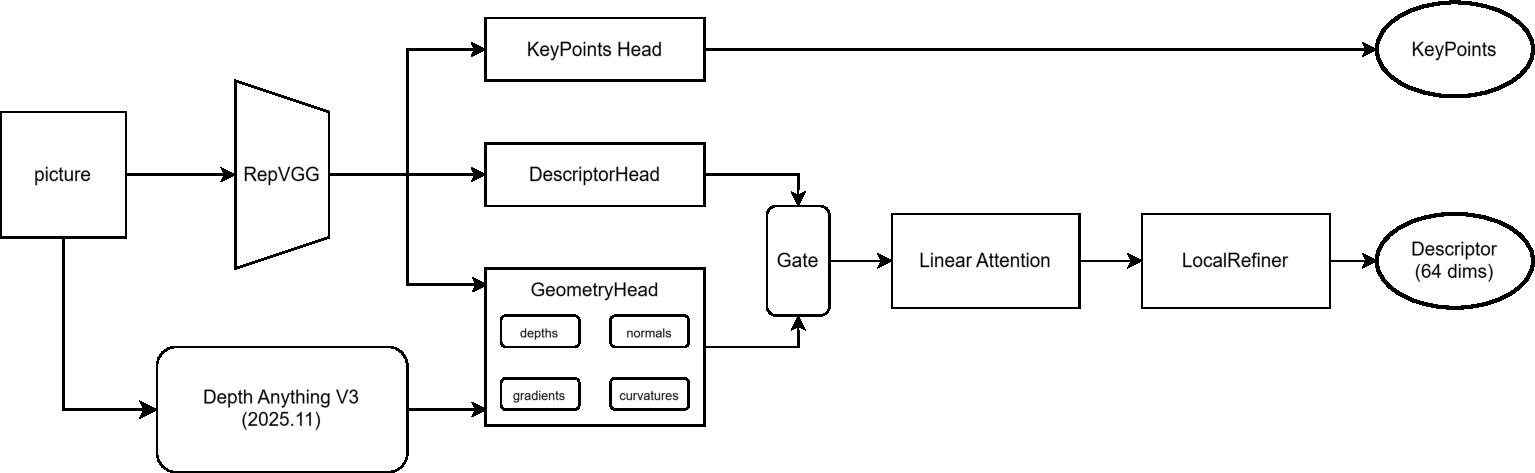
\includegraphics[width=0.9\textwidth]{./img/CurrentModel.pdf}
				\caption{GeoFeat 框架概览}
				\label{fig:GeoFeat}
			\end{figure}
			\par 如图\ref{fig:GeoFeat}，为了在准确性和速度之间取得更好的平衡，我们设计了一个轻量级的网络体系架构，该体系结构由三个主要模块组成：视觉特征提取器、几何特征提取器和融合模块。视觉特征提取器采用RepVGG轻量级卷积神经网络来提取图像的局部特征，而几何特征提取器则利用单目深度估计模型（如 Depth Anything V3）生成的深度图来计算深度梯度、法向量和曲率等几何特征。最后，融合模块通过无注意力机制将视觉和几何特征进行高效融合，以增强特征匹配的鲁棒性和准确性。
			\par 视觉特征提取器使用RepVGG网络结构，该结构在保持较低参数量的同时，能够有效地提取图像的局部特征。几何特征提取器则通过对单目深度图进行处理，计算出深度梯度、法向量和曲率等几何特征，这些特征能够提供关于场景结构的重要信息，有助于提升匹配的鲁棒性。融合模块采用无注意力机制，通过简单的连接和卷积操作将视觉和几何特征进行融合，从而增强了特征描述子的表达能力。	

			\textbf{Feature Encoding.}输入图像为$I \in \mathbb{R}^{H \times W \times 3}$，这里的$ W $ 和 $ H $分别表示图像的宽度和高度。在编码模块的功能编码中，我们采用了5层用于特征提取，所有块都是用3\texttimes3卷积层组成，然后是通过最大池化层进行下采样，横跨为2。最终，特征图的输出特征映射的空间分辨率为$\frac{W}{32} \times \frac{H}{32}$。通过视觉特征提取器得到视觉特征$F_v \in \mathbb{R}^{H' \times W' \times C_v}$。同时，单目深度估计模型生成的深度图$D \in \mathbb{R}^{H \times W}$经过处理后得到几何特征$F_g \in \mathbb{R}^{H' \times W' \times C_g}$。其中，$H'$和$W'$为特征图的空间尺寸，$C_v$和$C_g$分别为视觉和几何特征的通道数。
	\section{Experiments}
	\section{Conclusion}

\bibliographystyle{IEEEtran}
\bibliography{references}
\end{document}